% !TEX program = xelatex
% Template created by Jakob Eriksson (https://cs.uic.edu/profiles/jakob-eriksson/).
% Thanks to Jakob for creating+sharing 
\documentclass[11pt]{article}

% -----------------------------
% Page layout
% -----------------------------
\usepackage[margin=1in]{geometry}

% -----------------------------
% Font: CMU Serif (body) + CMU Sans Serif (headings)
% -----------------------------
\usepackage{fontspec}
\setmainfont{CMU Serif}
\setsansfont{CMU Sans Serif}

% -----------------------------
% Common utilities
% -----------------------------
\usepackage{microtype}
\usepackage{xcolor}
\usepackage{hyperref}
\usepackage{enumitem}
\usepackage{longtable}
\usepackage{array}
\usepackage{booktabs}

% Spacing
\usepackage{setspace}
\usepackage{graphicx}

% Headings with gray box
\usepackage[explicit]{titlesec}
\usepackage{tikz}
\usepackage[margin=1in]{geometry}


% -----------------------------
% Hyperlinks
% -----------------------------
\hypersetup{
  colorlinks=true,
  linkcolor=blue,
  urlcolor=blue,
  citecolor=blue
}

% Word-like paragraph behavior (tighter)
\setlength{\parindent}{0pt}
\setlength{\parskip}{0.18\baselineskip} % was 0.55
\setstretch{1.03}                      % was 1.12
\raggedbottom

% -----------------------------
% Lists (Word-like indentation and tight spacing)
% -----------------------------
\setlist[itemize]{leftmargin=1.25em, itemsep=0.15em, topsep=0.15em, parsep=0pt, partopsep=0pt}
\setlist[enumerate]{leftmargin=1.25em, itemsep=0.15em, topsep=0.15em, parsep=0pt, partopsep=0pt}

% -----------------------------
% Gray boxed section heading (Word-like)
% -----------------------------
\definecolor{uiclightgray}{RGB}{200,200,200}

\titleformat{\section}
  {\Large\bfseries\sffamily}
  {}
  {0em}
  {%
    \begin{tikzpicture}[baseline=(title.base)]
      \node[
        inner sep=8pt,
        fill=uiclightgray,
        draw=black,
        line width=0.8pt,
        text width=\dimexpr\textwidth-16pt\relax,
        align=left,
        anchor=west
      ] (title) {#1};
    \end{tikzpicture}%
  }
  []

% Control vertical spacing around section bars
\titlespacing*{\section}{0pt}{0.9\baselineskip}{0.6\baselineskip}

% Subsections: compact and bold like the Word template
\titleformat{\subsection}{\bfseries}{\thesubsection}{0.5em}{#1}
\titlespacing*{\subsection}{0pt}{0.8\baselineskip}{0.35\baselineskip}

% -----------------------------
% Table helpers
% -----------------------------
\newcolumntype{L}[1]{>{\raggedright\arraybackslash}p{#1}}

% Longtable spacing and padding similar to Word
\setlength{\LTpre}{0pt}
\setlength{\LTpost}{0pt}
\renewcommand{\arraystretch}{1.02}
\setlength{\tabcolsep}{6pt}

% -----------------------------
% Editable course metadata
% -----------------------------
\newcommand{\collegeName}{COLLEGE OF ENGINEERING, UIC}

\newcommand{\courseRubric}{CS}
\newcommand{\courseNumber}{377}
\newcommand{\courseTitle}{Ethical Issues in Computing}
\newcommand{\creditHours}{3}

\newcommand{\termSemesterYear}{Spring 2026}

\newcommand{\instructorName}{Jack Bandy}
\newcommand{\instructorEmail}{jxb@uic.edu}
\newcommand{\officeHours}{Monday and Wednesday, 10am-11:30am}
\newcommand{\officeHoursLocation}{CDRLC 3454}

\newcommand{\taOneName}{Abhijith Sreenivasan}
\newcommand{\taOneEmail}{asree5@uic.edu}
\newcommand{\taOneSectionDesignations}{12:30pm Section}


\newcommand{\taTwoName}{Elda Shatro}
\newcommand{\taTwoEmail}{eshatr2@uic.edu}
\newcommand{\taTwoSectionDesignations}{2:00pm Section}


\newcommand{\blackboardLinkText}{Canvas course}
\newcommand{\blackboardLinkUrl}{https://canvas.uic.edu}

\newcommand{\courseModalitySchedule}{%
\textbf{Course modality:} On campus \\
\textbf{Days/Times:} Mondays and Wednesdays \\
\textbf{Location/Link:} CDRLC 2411 \\
}

\newcommand{\catalogDescription}{%
Communication skills for computing professionals: presentation organization, visual
aides, delivery techniques, argument support. Ethical and societal issues in computing:
privacy, intellectual property and ownership, crime. \textbf{Prerequisite:} Credit or concurrent registration in CS 251.
}

\newcommand{\growthMindsetStatement}{%
Course materials and assignments can be complex and challenging, but they are crucial
to your intellectual and personal growth and development. There are times you may need
extra help. Students who attend class consistently, complete all assignments, thoughtfully
engage with feedback on work, develop good study strategies, visit the tutoring center,
and contact faculty when struggling can develop a thorough understanding of the course
material and ultimately succeed in the course.
}

\newcommand{\courseGoalsLearningOutcomes}{%
\begin{itemize}
  \item Develop an understanding of (personal and) professional responsibilities related to ethical, legal, security, and social issues in computing
  \item Practice describing current events in computing through classical ethical
perspectives (i.e. Deontological Ethics, Utilitarian Ethics, Virtue Ethics, Care Ethics)
  \item Identify recurring ethical challenges in computer science
  \item Develop a growth mindset for continuing (personal and) professional development, especially for effective decision-making and communication with different audiences
\end{itemize}

\textbf{Course requirement status:} CS 377 is \href{https://catalog.uic.edu/ucat/colleges-depts/engineering/cs/bs-cs/}{required} for a BS in Computer Science at UIC\\
\textbf{Topics overview:} Classical ethical theories (Virtue, Deontological, Utilitarian, Care Ethics); algorithmic feeds and content moderation; privacy and contextual integrity; inequality and algorithmic fairness; general cybersecurity; AI and large language models; intellectual property; environmental costs of computing.
}

\newcommand{\courseMaterials}{%
Copies of core readings will be provided to you via printed copies, web archives, and/or PDFs. Although there are no required books for this course, we will draw quite a bit from the following textbook:
\begin{itemize}
  \item \textit{Computing and Technology Ethics: Engaging through Science Fiction} by Emanuelle
        Burton, Judy Goldsmith, Nicholas Mattei, Cory Siler, and Sara-Jo Swiatek
\end{itemize}

Students will also make their own selections of different research papers, case studies,
books, and other materials to present and discuss in class.
}

\newcommand{\requiredTechnology}{%
The only technology you need is a web browser, from which you can access Canvas, course materials, and the Github repository for the class.
}

\newcommand{\copyrightStatement}{%
Please protect the copyright integrity of course materials. Particularly when it comes to materials in canvas, do not upload to third-party websites or share with anyone not enrolled in our course.
}

\newcommand{\gradingPolicy}{%
This class aims to use principles of student-centered teaching, also referred to as
``non-directive teaching,'' which de-emphasizes quantitative grading. This style focuses
on open-ended dialogue, project-based learning, and student curiosity, rather than
regurgitation and examinations. Still, in order to provide a final letter grade at the end of
the class, I will use the following combination of exercises:

\vspace{0.7em}
\noindent
{\renewcommand{\arraystretch}{1.30}%
\begin{tabular}{@{}p{0.72\linewidth}p{0.22\linewidth}@{}}
\toprule
& \textbf{Grade Proportion} \\
\midrule
\textbf{Out-of-class Exercises}             & \textbf{20\%} \\
\quad Food in your feed                     & \\
\quad Online account biopsy                 & \\
\quad Online account scrap doll             & \\
\quad Speculative fiction                   & \\
\quad Fairness definition                   & \\
\quad Personal ethical commitment           & \\
\midrule
\textbf{Read a Book}                        & \textbf{20\%} \\
\quad Book selection                        & \\
\quad 2-page book report or un-essay        & \\
\quad Peer instruction / book presentation  & \\
\quad Actually reading the book             & \\
\midrule
\textbf{In-class Group Exercises}           & \textbf{20\%} \\
\quad \textit{Expect about one per week}    & \\
\midrule
\textbf{Pre-Class Reflections}              & \textbf{20\%} \\
\quad \textit{Expect about one per week}    & \\
\midrule
\textbf{Attendance, Participation, Civility} & \textbf{20\%} \\
\bottomrule
\end{tabular}}

\vspace{0.9em}

You can expect the following correspondence between your percentage grade in the
course and your final letter grade, and the ``equivalent'' description from the registrar.

\vspace{0.5em}
\noindent
{\renewcommand{\arraystretch}{1.30}%
\begin{tabular}{|p{0.17\linewidth}|p{0.17\linewidth}|p{0.17\linewidth}|p{0.17\linewidth}|p{0.17\linewidth}|}
\hline
F              & D                & C        & B      & A         \\\hline
59\% or below  & 60--69\%         & 70--79\% & 80--89\% & 90--100\% \\\hline
Failure        & Poor but passing & Average  & Good   & Excellent \\\hline
\end{tabular}}
}

\newcommand{\lateWorkPolicy}{%
All due dates are listed in Canvas. For out-of-class exercises and pre-class reflections, late submissions may not be accepted after one week past the due date. For in-class group exercises, if you miss class that day, I will provide materials to make up the exercise.

If you anticipate difficulty meeting a deadline, please reach out \textit{before} the due date --- I am generally more flexible when contacted in advance.
}

\newcommand{\attendanceParticipationPolicy}{%
Showing up makes a big difference! As an instructor, I put a lot of effort into planning
classes that are meaningful, engaging, and valuable for your learning. As a student
enrolled in this course, I expect that you put a similar effort into attending class
meetings, arriving on time, and participating.

If you need to miss class due to illness, personal emergencies, and/or other unexpected situations, please notify the instructor as soon as possible so it can be recorded as an excused absence.

I will keep attendance on paper via roll call this semester and note any absences in Canvas. If you miss more than 50\% of class sessions, you will automatically fail the course. You are allowed three ``free''
absences without penalty, which do not have to be explicitly excused. If you miss a
fourth class without notifying the instructor, you will be contacted by the instructor.

The spring semester at UIC is fifteen weeks long (not including spring vacation), and
we meet Mondays and Wednesdays. With no class on Martin Luther King Jr.\ Day
(Monday, January 19th), we will have 29 total class periods.
}

\newcommand{\academicIntegrityPolicy}{%
As a student and member of the UIC community, you are expected to adhere to the Community Standards of academic integrity, accountability, and respect. Please review the UIC Student Disciplinary Policy for additional information; the UIC community standards for academic integrity are available at: \url{https://dos.uic.edu/community-standards/}

More concretely, my job and my goal in this course is to help you as you learn skills and knowledge that
will be valuable to you in your future courses, your career, and other areas of your life.
In line with UIC's mission to provide ``an environment in which research, learning, and scholarship can flourish and in which all endeavors are guided by academic and professional integrity,'' \textbf{the work you turn in for this class must be your own work}.

This does not mean that you need to complete all work in a bunker. Rather, you are
encouraged to discuss your ideas with friends and classmates, and to explore related
work (i.e.\ academic papers, blogs, video essays, forums, etc.). An important part of
scholarship is standing on the shoulders of giants,\footnote{Ironically, while this phrase
is often attributed to Isaac Newton in a letter from 1676, it was first recorded in John of
Salisbury's book \textit{Metalogicon} from 1159. I learned this from a blog post on
BookBrowse.com} (after all, we are in the City of the Big Shoulders\footnote{Sandburg,
Carl. ``Chicago.'' \textit{Poetry} (March 1914).}) and acknowledging whose shoulders we
stand upon. In other words, \textbf{cite your sources}!

\textbf{Please ask the instructor if you need clarity about academic integrity} for
specific exercises. When in doubt, it is always better to check with the instructor before proceeding.

I will reach out to you personally before submitting a report of academic misconduct.
}

\newcommand{\emailExpectations}{%
Students are responsible for all information instructors send to your UIC email and Canvas accounts. Faculty messages should be regularly monitored and read in a timely fashion.

While I do not closely monitor my email on Saturdays and Sundays, during the week, I generally respond to emails within 24 hours.
}

\newcommand{\scheduleDisclaimer}{%
This syllabus is intended to give the student guidance on what may be covered during the semester and will be followed as closely as possible. However, the instructor might alter this syllabus as course needs arise. I will communicate such changes in advance through in-class announcements and in writing via Canvas and/or email.
}

\newcommand{\disabilityAccommodation}{%
UIC is committed to full inclusion and participation of people with disabilities in all aspects of university life. If you face or anticipate disability-related barriers while at UIC, please connect with the Disability Resource Center (DRC)
at \url{https://drc.uic.edu}, via email at \href{mailto:drc@uic.edu}{drc@uic.edu}, or call (312) 413-2183 to create a plan for reasonable accommodations. To receive accommodations, you will need to disclose the disability to the DRC, complete an interactive
registration process with the DRC, and provide me with a Letter of Accommodation (LOA). Upon receipt of an LOA, I will gladly work
with you and the DRC to implement approved accommodations.
}

\newcommand{\religiousAccommodation}{%
Following campus policy, if you wish to observe religious holidays, you must notify me by the tenth day of the semester.
If the religious holiday is observed on or before the tenth day of the semester, you must notify me at least five days before you will be absent. Please submit this form by email with the subject heading: ``YOUR NAME: Requesting Religious Accommodation.''
}

\newcommand{\inclusiveCommunity}{%
UIC values diversity and inclusion. Regardless of age, disability, ethnicity, race, gender, gender identity, sexual orientation,
socioeconomic status, geographic background, religion, political ideology, language, or culture, we expect all members of this class
to contribute to a respectful, welcoming, and inclusive environment for every other member of our class. If aspects of this course
result in barriers to your inclusion, engagement, accurate assessment, or achievement, please notify me as soon as possible.
}

\newcommand{\namePronounUse}{%
If your name does not match the name on my class roster, please let me know as soon as possible.
My pronouns are he/him, and I welcome your pronouns if you would like to share them with me.
For more information about pronouns, see: \url{https://www.mypronouns.org/what-and-why}.
}

\newcommand{\communityAgreement}{%
Active participation is one of the most important ways you will learn in this course. I am
very aware that participation looks a little different for everyone, and will evaluate your
participation accordingly. Still, in general, an engaged student will:
\begin{itemize}
  \item come to class prepared, for example, by having completed pre-class reflections
\item contribute regularly to class activities and discussions
\item stay on-task during class
\item listen attentively to peers (no side conversations or unnecessary disruptions)
\item have an open mind and seek to understand (not judge and make assumptions)
\item be gracious and open to change in their ideas, arguments, and positions
\item assume goodwill in all interactions, even in disagreement
\item complete their work in a timely manner
\item reach out to the instructor if they start to fall behind
\end{itemize}
}

\newcommand{\contentNotices}{%
Our classroom provides an open space for a civil exchange of ideas which will intentionally include a variety of perspectives and positions. Some readings and other content may expose you to ideas, subjects, or views that may challenge you, cause you discomfort, or recall past negative experiences or traumas. I intend to discuss all subjects with dignity and humanity. If you would like me to be aware of a specific topic of concern, please email or visit me during office hours.
}

\newcommand{\resourcesSection}{%
We all need the help and the support of our UIC community. Please visit my office hours for course consultation and other academic or research topics.
For additional assistance, please contact your assigned college advisor and visit the support services available to all UIC students.

\subsection*{Academic Success}
\begin{itemize}
  \item Equity and Inclusion in Engineering Program
  \item UIC Library and UIC Library Research Guides
  \item Offices supporting the UIC undergraduate experience and academic programs
\end{itemize}

\subsection*{Wellness}
\begin{itemize}
  \item Access U\&I Care Program for assistance with personal hardships
  \item Campus Advocacy Network (Title IX): \href{mailto:TitleIX@uic.edu}{TitleIX@uic.edu} \quad and \quad \url{http://can.uic.edu/}
\end{itemize}

\subsection*{Safety}
\begin{itemize}
  \item UIC Safe App (please download for your safety)
  \item UIC Safety Tips and Resources
  \item Night Ride
  \item Emergency: Dial 5-5555 from a campus phone, or (312) 355-5555 from a cell phone
\end{itemize}
}

\begin{document}

% -----------------------------
% Centered header block
% -----------------------------
\begin{center}
  {\LARGE\bfseries \collegeName}\par
  \vspace{0.75em}
  {\Large\bfseries
    \courseRubric\ \courseNumber\quad
    \courseTitle\quad
    (\creditHours\ Credit Hours)
  }\par
  \vspace{0.5em}
    {\itshape ``Evil comes from a failure to think''   ---Hannah Arendt}\par
  \vspace{0.5em}

  {\large \termSemesterYear}\par
\end{center}

\vspace{0.9\baselineskip}

% -----------------------------
% Instructor and course details
% -----------------------------
\section*{Instructor \& Course Details}

% ===================================================================
% INSTRUCTOR & COURSE INFO TABLE
% ===================================================================
\noindent
\begin{tabular}{@{}p{0.16\linewidth}p{0.31\linewidth}p{0.19\linewidth}p{0.28\linewidth}@{}}
\textbf{Instructor} & Jack Bandy, Ph.D.                       & \textbf{Class Meeting} & Monday and Wednesday \\
\textbf{Email}      & \href{mailto:jxb@uic.edu}{jxb@uic.edu} &                        & CDRLC 2411           \\
\textbf{Office}     & CDRLC 3454                              & \textbf{Office Hours}  & Monday and Wednesday \\
                    &                                         &                        & 10am--11:30am        \\
                    &                                         &                        & CDRLC 3454           \\
                    &                                         &                        & Please schedule \href{https://calendar.app.google/P3weJsBwJYiEU6Fk6}{here} \\[1.2em]
\textbf{TA}         & \taOneName                              & \textbf{Section}       & \taOneSectionDesignations \\
\textbf{Email}      & \href{mailto:\taOneEmail}{\taOneEmail}  &                        &                      \\[0.4em]
\textbf{TA}         & \taTwoName                              & \textbf{Section}       & \taTwoSectionDesignations \\
\textbf{Email}      & \href{mailto:\taTwoEmail}{\taTwoEmail}  &                        &                      \\
\end{tabular}

\vspace{0.8\baselineskip}

\subsection*{Course Site}

\href{\blackboardLinkUrl}{\blackboardLinkText} --- Students are expected to log in to Canvas regularly to learn about any developments related to the course, upload assignments, and communicate with classmates.

% \courseModalitySchedule

% -----------------------------
% Course information
% -----------------------------
\section*{Course Information}

\subsection*{Catalog Course Description}
\catalogDescription

\subsection*{Dr.\ Bandy's Course Description}

What does it mean for Computer Scientists to be socially responsible? Billions of
people interact with computational systems every day for communication, amusement,
work, and more. Although many interactions appear to happen seamlessly, even the
most mundane human-computer interaction often has ethical implications related to
privacy, climate, power, inequality, public health, and more. To explore these ethical
implications, this course will survey classical perspectives of ethics (i.e.\ Deontological
Ethics, Utilitarian Ethics, Virtue Ethics, Care Ethics) and practice using them to interpret
real-world situations involving humans and computers. Students will engage with
recent scholarship about ethical issues in algorithmic decision-making, data
management, user interface design, software engineering, search engines, algorithmic
media feeds, large language models, and chatbots, to name some examples. Class
sessions will promote active engagement through peer teaching, small group
discussions, games, and more.


\subsection*{Course Goals and Learning Outcomes}
\courseGoalsLearningOutcomes

\subsection*{Required and Recommended Course Materials}
\courseMaterials

\subsection*{Growth Mindset}
\growthMindsetStatement

\subsection*{Required Technology}
\requiredTechnology

\subsection*{Respect for Copyright}
\copyrightStatement

% -----------------------------
% Course policies and classroom expectations
% -----------------------------
\section*{Course Policies \& Classroom Expectations}

\subsection*{Grading Policy and Point Breakdown}
\gradingPolicy

\subsection*{Tests}
There will be no tests or examinations in this class. I agree with Carl Rogers\footnote{\textit{On Becoming a Person}, Chapter 14} that life
itself offers enough examinations, and I hope the resources from this class help you meet life's tests with more confidence and satisfaction. See above for details regarding your final grade in the class.

\subsection*{Policy for Missed or Late Work}
\lateWorkPolicy

\subsection*{Attendance and Participation Policy}
\attendanceParticipationPolicy

\subsection*{Academic Integrity}
\academicIntegrityPolicy

\subsection*{Visitors}

This class may welcome visitors (i.e.\ prospective students, guest speakers, etc.) during
the semester. When possible, students will be notified in advance of guest attendance.

\subsection*{Email Expectations}
\emailExpectations

% -----------------------------
% Course schedule
% -----------------------------
\section*{Course Schedule}

{
% --- Schedule table: inside margins + taller rows + no underfull hbox warnings ---
\renewcommand{\arraystretch}{1.25}
\setlength{\extrarowheight}{1.5pt}
\setlength{\tabcolsep}{4pt}

\begin{longtable}{@{}
  >{\raggedright\arraybackslash}p{\dimexpr 0.10\linewidth-2\tabcolsep\relax}
  >{\raggedright\arraybackslash}p{\dimexpr 0.18\linewidth-2\tabcolsep\relax}
  >{\raggedright\arraybackslash}p{\dimexpr 0.42\linewidth-2\tabcolsep\relax}
  >{\raggedright\arraybackslash}p{\dimexpr 0.24\linewidth-2\tabcolsep\relax}
@{}}
\toprule
\textbf{Week} & \textbf{Date(s)} & \textbf{Topic(s) / In-Class Activities} & \textbf{Readings / Work Due} \\
\midrule
\endfirsthead

\toprule
\textbf{Week} & \textbf{Date(s)} & \textbf{Topic(s) / In-Class Activities} & \textbf{Readings / Work Due} \\
\midrule
\endhead

\midrule
\multicolumn{4}{r}{(continued)}\\
\endfoot

\bottomrule
\endlastfoot

1  & 1/12--1/14 & Warm-up activity; intro to Virtue Ethics & \\
2  & 1/19--1/21 & MLK Day (no class); intro to Deontological Ethics & Virtue Ethics Reflection \\
3  & 1/26--1/28 & Intro to Utilitarian Ethics and trolley problems; intro to Care Ethics & Reflection(s) \\
4  & 2/2--2/4   & Ethical theory review and case studies; Ethics in Algorithmic Feeds & Care Ethics Reflection; Select a Book; Food in your Feed; Ranking Exercise \\
5  & 2/9--2/11  & Algorithmic feeds; intro to Privacy and contextual integrity & In-class Privacy Policy Exercise \\
6  & 2/16--2/18 & Privacy and short story analysis; Dr.\ Bandy at SIGCSE & Here-and-Now Reflection; Online Account Biopsy \\
7  & 2/23--2/25 & Inequality, Justice, algorithmic fairness & Message in a Bottle Reflection; Online Account Scrap Doll \\
8  & 3/2--3/4   & Cybersecurity; medical and health technologies in AI & Speculative Fiction \\
9  & 3/9--3/11  & LLM ethical challenges & Reflection(s) \\
10 & 3/16--3/18 & Intellectual property & Fairness Definitions \\
11 & 3/23--3/25 & \textit{Spring Vacation --- No Classes} & \\
12 & 3/30--4/1  & Environmental computing impact; book presentations begin & Reflection(s) \\
13 & 4/6--4/8   & Book presentations & \\
14 & 4/13--4/15 & Book presentations & \\
15 & 4/20--4/22 & Book presentations & Personal Ethics Commitments \\
16 & 4/27--4/29 & Synthesis and conclusions & Book Report/Un-essay, Presentation \\

\end{longtable}
}

\subsection*{Disclaimer}
\scheduleDisclaimer

% -----------------------------
% Accommodations
% -----------------------------
\section*{Accommodations}

\subsection*{Disability Accommodation Procedures}
\disabilityAccommodation

\subsection*{Religious Accommodations}
\religiousAccommodation

% -----------------------------
% Classroom environment
% -----------------------------
\section*{Classroom Environment}

\subsection*{Inclusive Community}
\inclusiveCommunity

\subsection*{Name and Pronoun Use}
\namePronounUse

\subsection*{Guidelines for Participation and Classroom Conduct}
\communityAgreement

\subsection*{Content Notices}
\contentNotices

% -----------------------------
% Resources
% -----------------------------
\section*{Resources: Academic Success, Wellness, and Safety}

\subsection*{Student Wellbeing}

As a student at UIC, I hope you have come to enjoy the learning process and the life of
the mind, and I hope you enjoy this particular course. I also understand that life as a
college student can sometimes become distressing and overwhelming, which can
make it difficult to engage in class.

So, to help you succeed in this course (and in life), I encourage you to proactively care
for your body and mind. If you are struggling or anticipate any trouble attending class
or turning in assignments on time, please let me know as early as possible and I will do
whatever I can to help you prioritize your wellbeing.

Below are some of the many support services and resources available to all UIC
students:

\begin{itemize}
  \item Current Student Resources -- a one-stop shop for links to resources in the
        following categories: General, Academic, Student Support, Student Life,
        Technology, Health and Safety, and Getting Around Campus
  \item UIC Tutoring Resources
  \item UIC College of Engineering Tutoring Program
  \item The First-at-LAS academic success program for first-generation students
  \item Programs and initiatives supporting the UIC undergraduate experience and
        academic programs through the Student Success Initiative
  \item If you are experiencing personal hardships (e.g.\ personal and family
        emergencies, academics, interpersonal conflicts, personal safety, physical and
        mental health concerns, food or housing insecurity) and need resources and
        assistance, please reach out to the Student Assistance division
  \item Student Guide for Information Technology -- a comprehensive resource for UIC
        students describing the most commonly used IT services and tools supporting
        your success
  \item Navigating Health Resources at UIC -- explore the many resources that are on
        campus to support students' health and wellbeing and learn about how you can
        access them.
\end{itemize}

Importantly, if you are in immediate distress, please know the UIC Counseling Center
has crisis intervention services available 24 hours a day, 7 days a week. You can walk
into the Counseling Center during business hours to request to talk to a crisis
counselor, or you can call the Counseling Center main line at (312)~996-3490. If you are
calling outside of business hours, select ``2'' during the automated greeting to be
connected to a crisis counselor. You can find additional mental health resources and
services on the Counseling Center Website and the Student's Guide to Accessing
Behavioral Health Services at UIC.

For immediate crisis support outside of UIC, call or text ``9-8-8'' any time, 24 hours a
day, 7 days a week. Dialing 988 will connect you to a trained crisis professional. 988
offers services in Spanish, American Sign Language, and over 240 languages through
tele-interpretation services. The 988 website has an online chat feature, too.

\resourcesSection

\textit{The following are mostly boilerplate blurbs from our Academic Center for Excellence
(ACE).}\footnote{\url{https://teaching.uic.edu/cate-teaching-guides/syllabus-course-design/syllabus/}}

\subsection*{Support for Parenting Students}

UIC supports parenting students by providing affordable, high-quality childcare for
infants, toddlers, and young children, along with a comprehensive wraparound care
system, study-play areas across campus, accessible lactation rooms, year-round
family events, and more. For more information, contact Melinda Young
(\href{mailto:mmcghe2@uic.edu}{mmcghe2@uic.edu}) or visit the \href{https://littlesparks.uic.edu}{Little Sparks website}.


\textbf{The Writing Center} offers friendly and supportive tutors who can help you with
reading and writing in any of your courses, not just English. Tutors are ready to help
with other writing as well, such as job applications, personal statements, and resumes.
The tutor and you will work together to decide how to improve your writing. If you have
not started your assignment, that is OK. A tutor can help you brainstorm or make an
outline. Tutors understand that you might be using the Writing Center for the first time.
They are ready to guide you through your first session. You can choose to work with a
tutor in person or in real time over the internet using video, audio, or chat and a
whiteboard. For more information and to schedule an appointment, visit the Writing
Center website.

\textbf{The Math and Science Learning Center}, located in the Science and Engineering
South Building (SES) at 845 W.\ Taylor St.\ 3rd Floor, Room 247, is a meeting place for
students in Math, Biological Sciences, Chemistry, Earth and Environmental Sciences,
and Physics. At the MSLC, students can meet with graduate teaching assistants for
tutoring in 100-level courses, attend informal group study sessions with other students,
or meet up with friends to attend one of the workshops, seminars, or other activities
sponsored by the MSLC during the semester. Visit the MSLC website, call
312-355-4900, or email at \href{mailto:mslc@uic.edu}{mslc@uic.edu}.

\textbf{The Academic Center for Excellence (ACE)} can help if you feel you need more
individualized instruction in reading and/or writing, study skills, time management, etc.
Please call (312)~413-0031 or visit the Academic Center for Excellence (ACE) website
for more information.

\textbf{Emergency response guides} can be found at the Office of Preparedness and
Response. Please review and acquaint yourself with the guide and recommendations
for various emergency situations.

\textbf{Student Health Services} are available if you get sick during the semester. The Family
Medicine Center is committed to providing high-quality, student centered care and
services. It has attending physicians, residents, and nurse practitioners on staff to
provide the full range of primary health care services. The Family Medicine Center also
offers a limited set of health services at no additional cost to students who pay the
Student Health Service Fee (SHSF). Services include caring for an acute or urgent
illness (e.g., cold, strep throat, asthma attack, flu) or an injury. More information can be
found on the Family Medicine Center's Student Health webpage.

\textbf{Lastly}, since there is still space left on page ten, here is a picture of Hannah Arendt. She said that ``evil comes from a failure to think.'' If we are successful in this class, we will do some real thinking.

\vspace{2em}
\begin{center}
  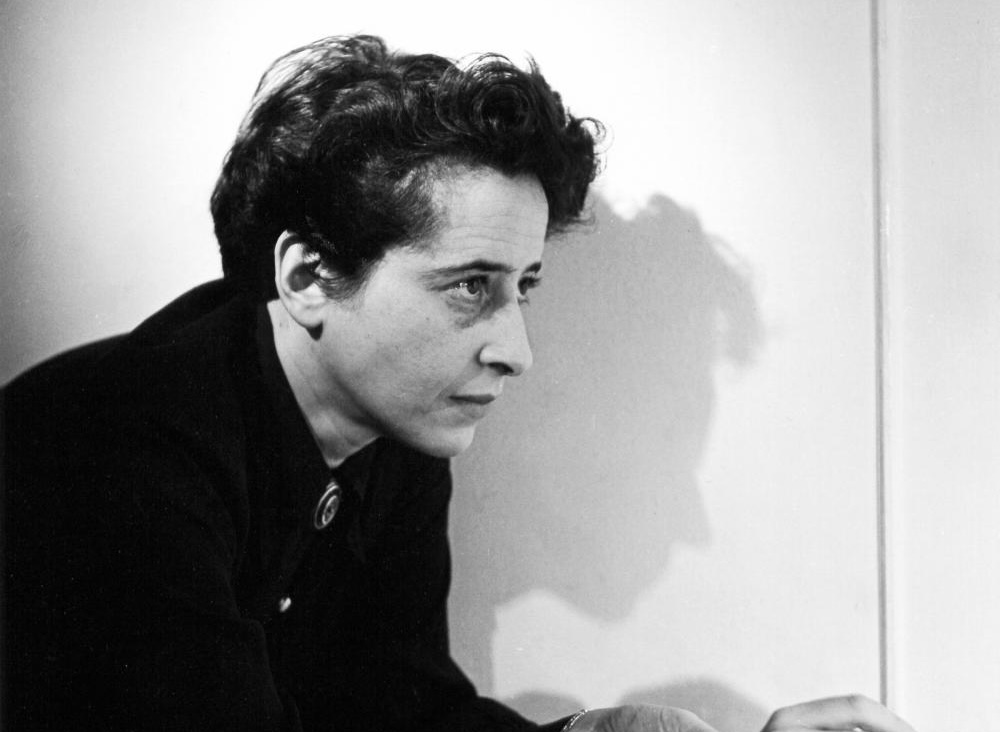
\includegraphics[width=0.55\textwidth]{arendt.jpg}\\[0.5em]
  \small Hannah Arendt, photographed on New Year's Day, 1944.\\
  \small \textcopyright\ Fred Stein/dpa/Corbis
\end{center}

\end{document}